\documentclass[dvisvgm,multi=true]{standalone}
\usepackage{mathmlcoresvg}
\begin{document}
%<figcaption><span>Figure 19: </span>Box model for the <code>circle</code>
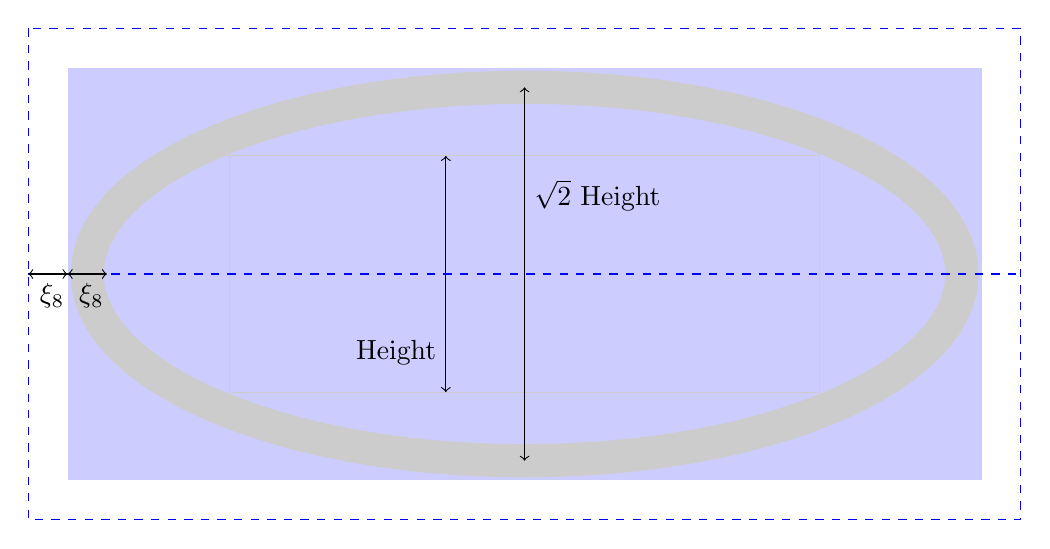
\begin{tikzpicture}[yscale=-1]

  \fill[blue!20]
  (-5.803300858899106,-2.621320343559643)
  rectangle (5.803300858899106,2.621320343559643);

  \MathMLBox{-3.75}{0}{1.5}{1}{red};

  \draw[black!20,line width=12]
  (0,0) ellipse (5.553300858899106 and 2.371320343559643);

  \draw[black!20]
  (-3.75,-1.5) rectangle (3.75,1.5);

  \draw[dashed,blue]
  (-6.303300858899106,-3.121320343559643)
  rectangle (6.303300858899106,3.121320343559643)
  (-6.303300858899106,0) -- (6.303300858899106,0);

  \draw[<->] (-6.303300858899106,0) --
  (-6,0)node[below]{$\xi_8$} --
  (-5.803300858899106,0);

  \draw[<->] (-5.803300858899106,0) --
  (-5.5,0)node[below]{$\xi_8$} --
  (-5.303300858899106,0);

  \draw[<->] (-1,-1.5) --
  (-1,1)node[left]{Height} --
  (-1,1.5);

  \draw[<->] (0,-2.371320343559643) --
  (0,-1)node[right]{$\sqrt{2}$ Height} --
  (0,2.371320343559643);

\end{tikzpicture}

\end{document}
